\chapter*{Itinéraire\markboth{Itinéraire}{}}
\section*{26 octobre 2014}
\vfill
\begin{center}

\includegraphics[width=\mywidth]{../wp-content/uploads/2014/10/7-drapeaux-1024x95.jpg}
\end{center}

\vfill
Le billet d'avion \og Tour du monde\fg\ est réservé, avec un départ le 8~février~2015 pour un retour le 20~décembre~2015.

\vfill
 Et voici les dates prévues dans chaque pays. Les billets d'avion étant flexibles, je peux changer les dates des vols à tout moment. 
\begin{itemize}
\item Chili : du 8 février au 1er avril 
\item Bolivie : du 2 avril au 29 avril 
\item Pérou : du 30 avril au 24 juin 
\item Équateur : du 25 juin au 12 juillet 
\item Japon : du 15 juillet au 30 août 
\item Chine : du 31 août au 25 octobre 
\item Inde : du 26 octobre au 20 décembre 
\end{itemize}
\vfill
\begin{center}
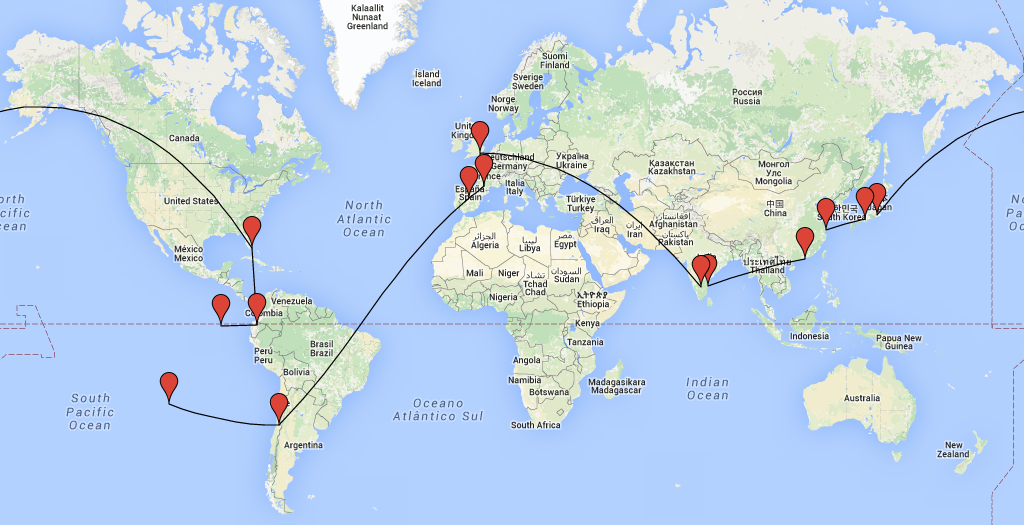
\includegraphics[width=\textwidth]{../wp-content/uploads/2016/01/carte_remi.png}
\end{center}
\vspace{-\topsep}
\vspace{-0.75mm}